\documentclass{article}

\usepackage{amsmath}
\usepackage{amsfonts}
\usepackage{tikz}
\usepackage{pgfplots}
\usepackage{graphicx}

\begin{document}

\section{Brachistochrone Curves}

A cycloid is parametrically described by the equations ($0 \leq s \leq 2 \pi$):

\begin{align}
	x(s) & = \frac C 2 \left( s - \sin s \right) \\
	y(s) & = \frac C 2 \left( \cos s - 1\right) 
\end{align}

The brachistochrone curve relating two points $A$ and $B$
	is a cycloid.
Let $A = (0,0)$, and $B = (\bar{x}, \bar{y})$.
I will show how to find $C$ so that the brachistochrone
		curve joints $A$ and $B$.

We must treat the cases $\bar{y} = 0$ and $\bar{y} \neq 0$ seperately.

\subsection{The case $\bar{y} = 0$}

If $\bar{y} = 0$, then either $C = 0$ or $\cos s = 1$.
If $C$ is zero, then $x(s)$ is zero for all $s$, and thus 
	cannot be equal to $\bar{x}$ for any choice of $s$.
Therefore, $\cos s = 1$.
Thus, $s = 0$ or $s = 2 \pi$.
If $s = 0$, then $x(s) = 0$.  
If $\bar{x} = 0$, we are done.
However, if $\bar{x} \neq 0$, then by process of elimination,
	if there is a solution, then $s = 2 \pi$.

We can now solve for $C$:

\begin{align}
\bar{x} & = \frac C 2 \left( 2 \pi - \sin ( 2 \pi) \right) \nonumber \\
	& = C \pi \nonumber \\
C & = \frac{\bar{x}}{ \pi }
\end{align}

\subsection{The case $\bar{y} \neq 0$}

If $\bar{y} \neq 0$, then neither $C$ nor $1 - \cos s$ is zero.
Therefore, we can write:

\begin{align}
\frac C 2 & = \frac {\bar{y}} {1 - \cos s}
\end{align}

If we combine this with the expression for $x(s)$, we can obtain the expression:

\begin{align}
\frac {\bar{x}} {\bar{y}} & = \frac {s - \sin s}{1 - \cos s}
\end{align}

If we can solve this expression for $s$, then we can substitute it into the 
	expression for $\bar{y}$ to obtain the value of $C$

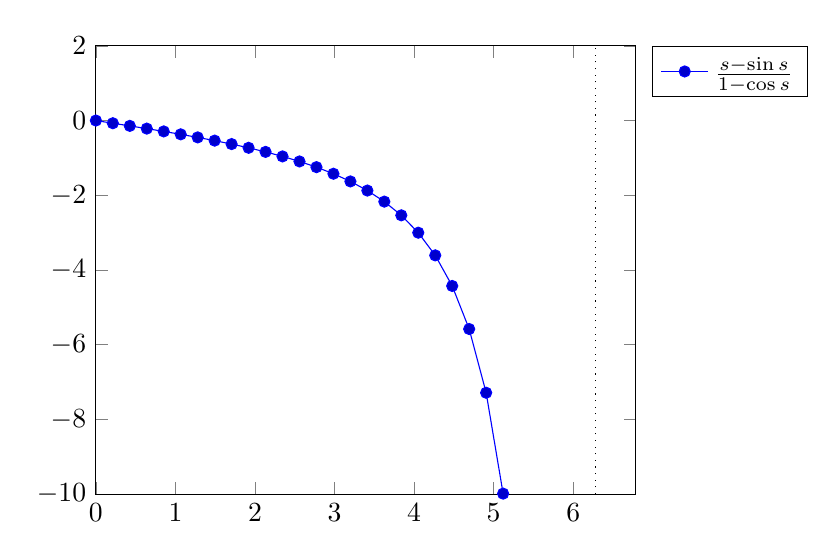
\begin{tikzpicture}
	\begin{axis}[domain=0:5.119, 
                 legend pos = outer north east,
                 xmin = 0,
                 xmax = 2*pi + 0.5,
                 ymin = -10.0,
                 ymax = 2.0]
	\addplot { (x - sin(deg(x)))/(cos(deg(x)) - 1) };
	\addplot[mark=none, dotted] coordinates { (2*pi, -10.0) (2*pi, 2.0)};
	\legend{$\frac {s - \sin s}{1 - \cos{s}}$}
	\end{axis}
\end{tikzpicture}

We solve for $s$ numerically when $\bar{y} \neq 0$:

\paragraph{}
\begin{tabular}{ l | l | l | l}
$\bar{x}$ & $\bar{y}$ & $s$ & $C$ \\
\hline
1 & 0 & $\pi$ & $\frac 2 {\pi - 1}$ \\
1 & 0.1 & 5.1198 & 0.3312 \\
1 & 0.2 & 4.5946 & 0.3579 \\
1 & 0.3 & 4.1763 & 0.3971 \\
1 & 0.4 & 3.8197 & 0.4497 \\
1 & 0.5 & 3.5084 & 0.5172 \\
1 & 0.6 & 3.2340 & 0.6013 \\
1 & 0.7 & 2.9910 & 0.7040 \\
1 & 0.8 & 2.7753 & 0.8275 \\
1 & 0.9 & 2.5833 & 0.9740 \\
1 & 1.0 & 2.4120 & 1.1458 \\
\end{tabular}

We plot the corresponding brachistochrone cycloids.

\paragraph{}
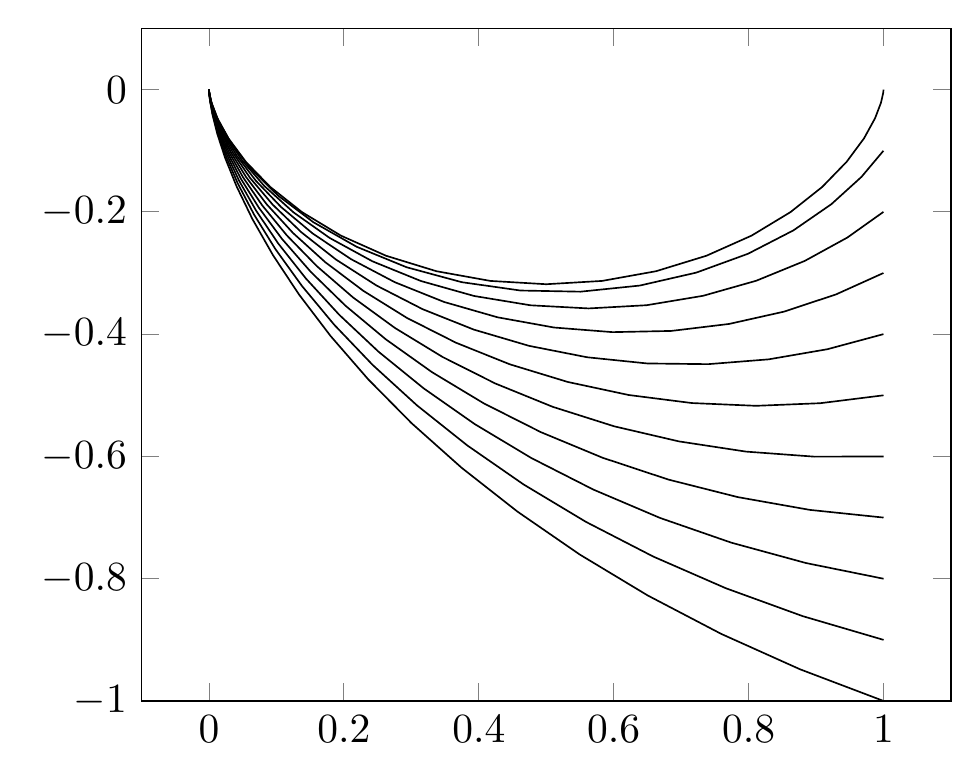
\begin{tikzpicture}[scale=1.5]
	\begin{axis}[xmin = -0.1,
                 xmax = 1.1,
                 ymin = -1.0,
                 ymax = 0.1]
		\addplot[domain=0:2*pi] ({(0.5/pi)*(x - sin(deg(x)))},{(0.5/pi)*(cos(deg(x)) - 1)});
		\addplot[domain=0:5.1198, samples = 20] ({(0.3312/2)*(x - sin(deg(x)))},{(0.3312/2)*(cos(deg(x)) - 1)});
		\addplot[domain=0:4.5946, samples = 20] ({(0.3579/2)*(x - sin(deg(x)))},{(0.3579/2)*(cos(deg(x)) - 1)});
		\addplot[domain=0:4.1763, samples = 20] ({(0.3971/2)*(x - sin(deg(x)))},{(0.3971/2)*(cos(deg(x)) - 1)});
		\addplot[domain=0:3.8197, samples = 20] ({(0.4497/2)*(x - sin(deg(x)))},{(0.4497/2)*(cos(deg(x)) - 1)});
		\addplot[domain=0:3.5084, samples = 20] ({(0.5172/2)*(x - sin(deg(x)))},{(0.5172/2)*(cos(deg(x)) - 1)});
		\addplot[domain=0:3.2340, samples = 20] ({(0.6013/2)*(x - sin(deg(x)))},{(0.6013/2)*(cos(deg(x)) - 1)});
		\addplot[domain=0:2.9910, samples = 20] ({(0.7040/2)*(x - sin(deg(x)))},{(0.7040/2)*(cos(deg(x)) - 1)});
		\addplot[domain=0:2.7753, samples = 20] ({(0.8275/2)*(x - sin(deg(x)))},{(0.8275/2)*(cos(deg(x)) - 1)});
		\addplot[domain=0:2.5833, samples = 20] ({(0.9740/2)*(x - sin(deg(x)))},{(0.9740/2)*(cos(deg(x)) - 1)});
		\addplot[domain=0:2.4120, samples = 20] ({(1.1458/2)*(x - sin(deg(x)))},{(1.1458/2)*(cos(deg(x)) - 1)});
	\end{axis}
\end{tikzpicture}

\section{Beachgoers Problem (feat. Sascha Hernandez)}

Consider the problem of finding the best location for relaxing on a beach.
Some parts of the beach are naturally more attractive than others,
	because of scenic views, proximity to parking, and lack of seagulls.
Additionally, the higher the density of people in a certain area,
	the less attractive it becomes.

We assume that the ``innate attractiveness'' of the beach at $x$ is measured
	by a function $N(x)$, and to find the actual attractiveness, $N(x)$
	is scaled by a crowding penalty $C(q(x))$, which depends on 
	$q(x)$, the total number of beachgoers at $x$.
For this example, we will use the following values of $N$ and $C$:

\begin{align}
	N(x) & = e^{-\left( x - \frac12\right)^2} \\
	C(q) & = \frac 1 {1 + q^2}
\end{align}

The attractiveness is thus given by:

\begin{align}
	A(x) & = N(x) C( q( x) )
\end{align}

\subsection{Individual Choice}

If each beachgoer chooses their spot individually, and only sees the segments
	of beach immediately surrounding them, then if the distribution
	of people along the beach is in equilibrium, the attractiveness must be 
	constant everywhere.
Therefore, for a choice of attractiveness $A$, the density of people
	on the beach is given by:

\begin{align}
	q(x) & = C^{-1} \left( \frac A {N(x)} \right)
\end{align}

if $C^{-1}$ exists.

\subsubsection{Finding $C^{-1}$}

A function is \emph{$C^{-1}$ at $q$} if $C(C^{-1}(q)) = q$.
We can therefore try to find functions which are $C^{-1}$ for positive $q$.

\begin{align}
q & = C(C^{-1}(q)) \nonumber \\
	& = \frac 1 {1 + \left(C^{-1}(q)\right)^2 } \nonumber \\
1 + \left(C^{-1}(q)\right)^2 & = \frac 1 q \nonumber \\
C^{-1}(q) & = \pm \sqrt{ \frac 1 q - 1 }
\end{align} 

We choose the positive branch of the square root in this case, because
	the population density at $x$ must be positive.
Note that there is a unique inverse, so we can proceed.

We can now find $q(x)$ for a given value of $A$:

\begin{align}
q(x) & = \sqrt{ \frac {N(x)} A - 1 }
\end{align}

Note that this is real everywhere because $A = N(x) C(q(x))$ everywhere,
	so $\frac A {N(x)} = C(q(x))$, and we have chosen $C(q(x))$ so 
	that it is less than or equal to one eveywhere.
Therefore, $\frac {N(x)} A$ is greater than or equal to one everywhere.

\subsubsection{Finding the Equilibrium Distribution for a Fixed Population}

Suppose we want the population size to be fixed, i.e., we require
	that for a constant $P$, $\int_0^1 q(x) dx = P$.
We will first rephrase our expression for $q(x)$ so that it is in terms
	of $q(0)$ and not $A$.
Since the value of $A$ is constant, and $A(0) = N(0) C(q(0))$,
	then

\begin{align}
	A & = \frac{N(0)}{1 + q(0)^2}
\end{align}

Substituting this into the expression for $q(x)$ yields:

\begin{align}
	q(x) & = \sqrt{ \frac{N(x)}{N(0)} \left( 1 + q(0)^2 \right) - 1 }
\end{align}

\subsubsection{Deriving a Differential Equation}

In situations when $C^{-1}$ is not well-behaved, it may be worthwhile
	to find a differential equation for $q(x)$.
For individual equilibrium to hold, the derivative of the attractivness
	must be zero everywhere.

\begin{align}
	0 & = \frac d {dx} A(x) \nonumber \\
	0 & = \frac d {dx} \left(  N(x) C( q( x ) ) \right) \nonumber \\
	0 & = \frac {dN}{dx}(x) C( q(x) ) + N(x) C'(q(x))\frac {dq}{dx} \nonumber 
\end{align}

Assuming that $N(x) \neq 0$ everywhere, and $C'(q(x)) \neq 0$ everywhere,
	then $q(x)$ must satisfy the following differential equation:

\begin{align}
	\frac {dq}{dx}(x) 
		& = - \frac
			{ \frac {dN}{dx}(x) C( q(x) )}
			{ N(x) C'(q(x)) } \label{eq-dqdx-choice}
\end{align}

\subsection{Finding the Distribution for a fixed population}

%	If we want to specify a total population, and derive the distribution
%		of beachgoers along the beach, we can define the definite integral
%		of $q(x)$ in the following manner:
%	
%	\begin{align}
%		Q(x) & = \int_0^x q(\xi) d\xi
%	\end{align}
%	
%	Note that $Q'(x) = q(x)$.
%	Therefore, (\ref{eq-dqdx-choice}) becomes the second-order differential
%		equation:
%	
%	\begin{align}
%		Q''(x) & = - \left( \frac {N'(x)}{N(x)} \right) 
%			\left( \frac{ C(Q'(x)) }{ C'(Q'(x))} \right)
%	\end{align}
%	
%	To obtain $q(x)$ for a fixed population $P$, $Q(x)$ is solved as a two-point
%		boundary-value problem, with boundary conditions $Q(0) = 0$ and
%		$Q(1) = P$.

Since we know the equation for $q(x)$, for a given initial population
	density $q(0)$, we can vary $q(0)$ in order to get a desired population.
We show a plot of the total population $P$ as a function of the population
	at the boundary, $q(0)$.
At an initial population of zero, the total popualation is $0.412104$.
Obviously, the initial population cannot go below zero.
Therefore this is the lowest population I could get it to work at.

\subsubsection{Extension to Lower Populations}

Obviously, our model should predict what happens on the beach when
	the total population is smaller than $0.412104$.
We need our population to be nonnegative.
Our basic assumption is that people move to regions of greater desirability.
If there are not enough people, however, then some regions may not be
	as desirable as others no matter how empty they are.
These regions should be empty.
The boundary between these regions and the populated regions will
	be when $q(x) = 0$, so that there is a continuous transition
	between the populated and unpopulated regions.

For our case, $q(x)$ is given by:

\begin{align}
	q(x) & = \sqrt{ \frac{N(x)}{A} - 1} \nonumber \\
	N(x) & = e^{-(x - 0.5)^2} \nonumber
\end{align}

Therefore, there is a boundary between an inhabited and an uninhabited
	zone when $q(x) = 0$, or when:

\begin{align}
	0 & = q(x) \nonumber \\
	& = \sqrt{ \frac{N(x)}{A} - 1} \nonumber \\
	N(x) & = A 
\end{align}

To determine at what points the population starts and stops, we need 
	to invert $N(x)$.

\begin{align}
	N^{-1}(A) & = \frac 12 \pm \sqrt{ - \log A } 
\end{align}

To determine the total population, we need to integrate between 0 and
	1 if they both do not have population density zero, 
	or between the two boundary points if 0 and 1 have population density
	zero.
To determine the value of $A$ at which we must switch strategies,
	we can compute the value of $A$ at which $N(0) = N(1) = A$.
This value of $A$ is $e^{- \frac 1 4}$.
Therefore, when $A < e^{- \frac 1 4}$, we can assume that the population
	is nonzero all the way up to the boundary.
However, when $A > e^{- \frac 1 4}$, we must only integrate between
	$ \frac 1 2 - \sqrt{ - \log A}$ and $\frac 1 2 + \sqrt{ - \log A}$.

We can summarize this with a function for total population as a function
	of the attractiveness of the inhabited areas:

\begin{align}
P(A) & = \begin{cases}
\int_0^1 \sqrt{ \frac{N(x)}{A} - 1} & A \leq e^{- \frac 1 4} \\
\int_{\frac 1 2 - \sqrt{ - \log A}}^{\frac 12 + \sqrt{ -\log A}}
	\sqrt{ \frac{N(x)}{A} - 1}
	& A > e^{- \frac 1 4} 
\end{cases}
\end{align}

We can plot $P(A)$, which was found from numerical integration in OCTAVE:

\pgfplotstableread[col sep = comma]{total_population_individual.csv}\Pindividual
\begin{tikzpicture}
	\begin{axis}[
		xmin = -0.1, xmax = 1.1,
		ymin = -0.1, ymax = 12.0,
		xlabel = {$A$, beach attractiveness (where inhabited)},
		ylabel = {$P$, total population},
		title = {Total Population given fixed Beach Attractiveness at Equilibrium}
	]
		\addplot[mark=""] table[x index = {0}, y index = {1}]{\Pindividual};
	\end{axis}
\end{tikzpicture}

To see how varying the population of the beach affects the overall happiness,
	we plot $A(P)$, the inverse.

\paragraph{}
\begin{tikzpicture}
	\begin{axis}[
		xmin = -0.1, xmax = 12.0,
		ymin = -0.1, ymax = 1.1,
		ylabel = {$A$, beach attractiveness (where inhabited)},
		xlabel = {$P$, total population},
		title = {Average Beach Attractiveness given Beach Population (Individual Movement)}
	]
		\addplot[mark=""] table[x index = {1}, y index = {0}]{\Pindividual};
	\end{axis}
\end{tikzpicture}

Notice that the beach becomes dramatically less attractive the more
	crowded it becomes.

We have numerically solved for the enjoyment $A$ associated with some given 
	values of $P$, which we present below:

\paragraph{}
\begin{tabular}{ l | l}
Population & Enjoyment ($A$) \\
\hline
0.05 & 0.9689 \\
0.10 & 0.9390 \\
0.15 & 0.9105 \\
0.20 & 0.8831 \\
0.25 & 0.8568 \\
0.30 & 0.8316 \\
0.35 & 0.8074 \\
0.40 & 0.7842 \\
0.45 & 0.7597 \\
0.50 & 0.7323 \\
0.55 & 0.7037 \\
0.60 & 0.6746 \\
0.65 & 0.6454 \\
0.70 & 0.6165 \\
0.75 & 0.5881 \\
0.80 & 0.5605 \\
0.85 & 0.5338 \\
0.90 & 0.5081 \\
0.95 & 0.4835 \\
1.00 & 0.4600 
\end{tabular}

\paragraph{}
To illustrate some typical population densities, we plot $q(x)$ for each
	value of $A$ in the above table.
The lower curves are for the higher satisfaction $A$.

\pgfplotstableread[col sep = comma]{individual-choice-qs.csv}\curves
\paragraph{}
\begin{tikzpicture}
	\begin{axis}[
		xmin = 0.0, xmax = 1.0,
		xlabel = {$x$, position on beach},
		ylabel = {$q(x)$, population density at $x$},
		title = {Population Densities under Free Movement for different total populations},
		]
		\addplot[mark=""] table[x index = 0, y index = 20]{\curves};
		\addplot[mark=""] table[x index = 1, y index = 21]{\curves};
		\addplot[mark=""] table[x index = 2, y index = 22]{\curves};
		\addplot[mark=""] table[x index = 3, y index = 23]{\curves};
		\addplot[mark=""] table[x index = 4, y index = 24]{\curves};
		\addplot[mark=""] table[x index = 5, y index = 25]{\curves};
		\addplot[mark=""] table[x index = 6, y index = 26]{\curves};
		\addplot[mark=""] table[x index = 7, y index = 27]{\curves};
		\addplot[mark=""] table[x index = 8, y index = 28]{\curves};
		\addplot[mark=""] table[x index = 9, y index = 29]{\curves};
		\addplot[mark=""] table[x index = 10, y index = 30]{\curves};
		\addplot[mark=""] table[x index = 11, y index = 31]{\curves};
		\addplot[mark=""] table[x index = 12, y index = 32]{\curves};
		\addplot[mark=""] table[x index = 13, y index = 33]{\curves};
		\addplot[mark=""] table[x index = 14, y index = 34]{\curves};
		\addplot[mark=""] table[x index = 15, y index = 35]{\curves};
		\addplot[mark=""] table[x index = 16, y index = 36]{\curves};
		\addplot[mark=""] table[x index = 17, y index = 37]{\curves};
		\addplot[mark=""] table[x index = 18, y index = 38]{\curves};
		\addplot[mark=""] table[x index = 19, y index = 39]{\curves};
%		\foreach \index in {0, ..., 19} {%
%			\addplot[mark=""] table[x index = {\index}, y index = {20+\index}]{\curves};
%		}
	\end{axis}
\end{tikzpicture}

\subsection{Average Satisfaction}

It is natural to define the average satisfaction for a beachgoer
	for each particular distribution:

\begin{align}
S[q] & = \frac{ \int_0^1 N(x) C(q(x)) q(x) dx}{\int_0^1 q(x) dx}
\end{align}

Notice that if $q(x)$ is such that $A(x)$ is constant where $q$ is nonzero, then:

\begin{align}
S[q] & = \frac{ \int_0^1 A q(x) dx}{\int_0^1 q(x) dx} \nonumber \\
	& = A
\end{align}

Therefore, the average happiness is $A$.

\subsection{A Benevolent Dictator maximizes Average Happiness}

Suppose a benevolent dictator is attempting to maximize average happiness.
Then, if $\bar{A}(x) = N(x) C(q(x)) q(x)$ is the density of average happiness
	everywhere, then $\bar{A}(x)$ must be a constant.
Therefore, for some constant $B$,

\begin{align}
	B & = N(x) C(q(x)) q(x)
\end{align}

From this we can derive a differential equation:

\begin{align}
	0 & = \frac {d}{dx} \left[ N(x) C(q(x)) q(x) \right] 
\end{align}

This differential equation can be put in standard form:

\begin{align}
	q'(x) & = - \left( \frac {N'(x)}{N(x)} \right) \frac{ C(q(x)) q(x) }{C'(q(x))q(x) + C(q(x))}
\end{align}

(This isn't yours?  I'm not sure how to get the one given)

\subsection{Derivation}

I skipped this section.

\subsection{Solutions}

The differential equation was integrated for total populations ranging from 
	0.05 to 1.0

\includegraphics[width=\textwidth]{dictator-distributions.png}

\begin{tabular}{l | l | l }
Population & Dictatorial Satisfaction & Individual Choice Satisfaction\\
\hline
0.05&0.969551949716576 & 0.9689\\
0.1&0.9410909123993225 & 0.9390\\
0.15&0.9148666447945552 & 0.9105 \\
0.2&0.8897254121698162 & 0.8831 \\
0.25&0.8650746522441468 & 0.8568\\
0.3&0.8403522597511855 & 0.8316 \\
0.35&0.8146672860405727 & 0.8074 \\
0.4&0.7875000139626287 & 0.7842 \\
0.45&0.7591273355506913 & 0.7523 \\
0.5&0.7299151727699459 & 0.7323 \\
0.55&0.7002400142580769 & 0.7037 \\
0.6000000000000001&0.6704534714129022 & 0.6746 \\
0.6500000000000001&0.6408657300334135 & 0.6454 \\
0.7000000000000001&0.6117388969061799 & 0.6165 \\
0.7500000000000001&0.5832860501461835 & 0.5881 \\
0.8&0.5556736577186869 & 0.5605\\
0.8500000000000001&0.5290258017829101 & 0.5338 \\
0.9000000000000001&0.5034296789487028 & 0.5081 \\
0.9500000000000001&0.4789408404669266 & 0.4835 \\
1&0.4555887321040328 & 0.4600 \\
\end{tabular}

Obviously something is wrong, since the dictatorial satisfaction is not always
	larger than the individual choice satisfaction!

\section{Cell Phone Walk}

(Reprint from earlier in the semester)
Suppose a cell tower generates the following reception profile 
	(\ref{eq:cell-reception}).

\begin{align}
s(x,y) & = \begin{cases}
	20 - 5 (x^2 + y^2) & \text{if $x^2 + y^2 < 4$} \\ 
	0 & \text{otherwise} \\ \end{cases} \label{eq:cell-reception}
\end{align}

Suppose the caller needs to walk from point $a$ to point $b$ in at least $T$ minutes, 
	and the caller's speed of motion cannot exceed $V$.
What path through the plane has the best average reception?

Let's say that a path is a function $\gamma$ which satisfies:

\[ \gamma : [0,T] \to \mathbb{R}^2 \]
\[ \gamma(0) = a \]
\[ \gamma(T) = b \]

Let's define $x(t)$, $y(t)$ by:

\begin{align}
\gamma(t) = (x(t), y(t))
\end{align}

\subsection{Extremal Cases}

Since $s$ has a maximum at $(0,0)$, if we have enough time to go to the maximum
	and back, this will have the best average reception.
Going to the maximum from $(-2,0)$ is 2 distance units away, and going from
	the maximum to $(0,-2)$ is also 2 distance units away.
Therefore, if we have the time to cover 4 distance units, we can go straight to the
	maximum.
We can travel $V T$ distance units total if we always move at our maximum speed.
Therefore, if $V T \geq 4$, then we will be able to go right to the maximum.

Since we can travel only $ V T$ distance units total, if this is smaller than 
	the distance from $a$ to $b$, then there will be no way to move in the 
	desired way.
The distance from $(-2,0)$ to $(0,2)$ is $2 \sqrt{2}$ distance units, so therefore,
	if $V T < 2 \sqrt{2}$, then there will be no solution.

The interesting case is therefore when $2 \sqrt{2} < V T < 4$, when a solution
	exists, but it is not possible to go directly to the maximum.

\subsection{Minimizing a Functional (Cartesian Coordinates)} 

I first derive the differential equations for a minimized functional
	in cartesian coordianates to analyze singularities and demonstrate
	the validity of the method.
I will then re-derive them in polar coordiantes, and use those.

Suppose $2 \sqrt{2} < V T < 4  $.
Then, we need to determine the shape of the path $\gamma$ to maximize the
	average reception (\ref{eq:avg-reception}):

\begin{align}
\langle s \rangle = \frac{\int_0^T s(x(t),y(t)) dt}{\int_0^T dt} 
	\label{eq:avg-reception}
\end{align}

If we have a path, and on some subsection of that path, we are not moving at
	the maximum speed, we can increase the total average reception
	by traversing this path at full speed, and then going towards the center
	and turning around.
Therefore, all paths which do not move at the maximum allowed speed are not 
	optimal.

Therefore, we conclude that:

\begin{align}
\sqrt{\frac{dx}{dt}^2 + \frac{dy}{dt}^2} & = V
\end{align}

Suppose $y(t) = f(x(t))$.
This is a non-trivial assumption.
It is assuming that optimal paths go only one way in the x direction.
It is true in this case because if a path does go backwards in the
	x direction, one can make a better path simply by waiting where you 
	are and then skipping ahead.
Then,

\begin{align}
V & = \sqrt{\frac{dx}{dt}^2 + \frac{df}{dx}^2\frac{dx}{dt}^2}  \nonumber \\
V & = \frac{dx}{dt} \sqrt{ 1 + \frac{df}{dx}^2}  \nonumber \\
dt & = \frac{1}{V} \sqrt{1 + \frac{df}{dx}^2} dx \label{eq:dt-to-dx}
\end{align}

Therefore we can rewrite the expression for $\langle s \rangle$:

\begin{align}
\langle s \rangle & = \int_{x_a}^{x_b} 
	\frac{s(x,f(x))}{VT} \sqrt{1 + \frac{df}{dx}^2} dx \label{eq:path-integral}
\end{align}

Now that we're integrating over $x$, we don't automatically have the constraint
	on the path length anymore.
We want to maximize $\langle s \rangle$, but subject to the constraint that the
	path length is $V T$.
This constraint can be written as a functional of $f$:

\begin{align}
V T & = \int_{x_a}^{x_b} \sqrt{1 + \frac{df}{dx}^2} dx \label{eq:constraint-on-lambda}
\end{align}

To find the $f$ which extremizes $\langle s \rangle$ with the desired arclength,
	we use a lagrange multiplier $\lambda$, and look for optimal solutions
	to the following functional.

\begin{align}
S[f] & = \frac{1}{VT} \int_{x_a}^{x_b} \left( s(x, f(x)) + \lambda \right)
	\sqrt{1 + \frac{df}{dx}^2} dx \label{eq:action}
\end{align}

Let $n(x, f(x)) = s(x, f(x)) + \lambda)$.
This functional is of the form of an integral $\int_a^b \mathcal{L}(x,f(x),f'(x)) dx$,
	so therefore every $f$ which extremizes $S$ satisfies the following
	instance of the euler-lagrange equation:

\begin{align}
\mathcal{L} & = n(x, f(x)) \sqrt{1 + \frac{df}{dx}^2} \\
\frac{d}{dx} \left( \frac{\partial \mathcal{L}}{\partial \frac{df}{dx}} \right)
	& = \frac{\partial \mathcal{L}}{\partial f} \nonumber 
\end{align}

In this case, this becomes:

\begin{align} 
\frac{d}{dx} \left( \frac{n(x, f(x)) \frac{df}{dx}}{\sqrt{1 + \frac{df}{dx}^2}} \right)
	& = \frac{\partial n}{\partial y} \sqrt{1 + \frac{df}{dx}^2} \nonumber\\
\frac{\partial n}{\partial y} \sqrt{1 + \frac{df}{dx}^2} 
& = \frac{\frac{\partial n}{\partial y} \frac{df}{dx} 
		+ \frac{\partial n}{\partial x} 
		+ n(x,f(x)) \frac{\partial^2 f}{\partial x^2}}
	{\sqrt{1 + \frac{df}{dx}^2}}
	- \frac{n(x,f(x)) \frac{df}{dx}^2 \frac{d^2f}{dx^2}}
		{\left( 1 + \frac{df}{dx}^2 \right)^{\frac32}} \nonumber\\
\frac{\partial n}{\partial y} \left(1 + \frac{df}{dx}^2 \right)^2
& = \left( \frac{\partial n}{\partial y} \frac{df}{dx} 
		+ \frac{\partial n}{\partial x} 
		+ n(x,f(x)) \frac{d^2 f}{d x^2} \right)
	\left(1 + \frac{df}{dx}^2\right)
	- n(x,f(x)) \frac{df}{dx}^2 \frac{d^2f}{dx^2} \nonumber\\
\frac{d^2 f}{dx^2}
& = \frac{\frac{\partial n}{\partial y}}{n} \left(1 + \frac{df}{dx}^2 \right)^2
-	\left( \frac{\frac{\partial n}{\partial y}}{n} \frac{df}{dx} 
		+ \frac{\frac{\partial n}{\partial x}}n \right)
	\left(1 + \frac{df}{dx}^2\right) \nonumber\\
\frac{d^2 f}{dx^2}
& = \left( 1 + \frac{df}{dx}^2 \right) \left(
		\frac{\frac{\partial n}{\partial y}}n
		\left( 1 - \frac{df}{dx} + \frac{df}{dx}^2 \right) 
		- \frac{\frac{\partial n}{\partial x}}n
	\right) \nonumber
\end{align}

Since there are two boundary conditions, for each choice of $\lambda$ there
	exists a unique $f$ such that $f(x_b) = y_b$ and $f(x_a) = y_a$.
Furthermore, we know that $n = s(x,f(x)) - \lambda$ should never be zero
	within any area where we expect the path to be.


\subsection{Minimizing a Functional (Polar Coordinates)} 
Suppose $2 \sqrt{2} < V T < 4  $.
We can also express $\gamma(t) = (r(t), \theta(t))$ in ploar coordinates.
Then, we need to determine the shape of the path $\gamma$ to maximize the
	average reception (\ref{eq:avg-reception-polar}):

\begin{align}
\langle s \rangle = \frac{\int_0^T s(r(t),\theta(t)) dt}{\int_0^T dt} 
	\label{eq:avg-reception-polar}
\end{align}

Since, as before, we are always moving at the maximum speed, we conclude that:

\begin{align}
\sqrt{\frac{dr}{dt}^2 + r^2\frac{d\theta}{dt}^2} & = V
\end{align}

Suppose $r(t) = f(\theta(t))$.
Then,

\begin{align}
V & = \sqrt{\frac{df}{d\theta}^2\frac{d\theta}{dt}^2 + f(\theta)^2\frac{d\theta}{dt}^2}  \nonumber \\
V & = \frac{d\theta}{dt} \sqrt{ f(\theta)^2 + \frac{df}{d\theta}^2}  \nonumber \\
dt & = \frac{1}{V} \sqrt{f(\theta)^2 + \frac{df}{d\theta}^2} dx \label{eq:dt-to-dtheta}
\end{align}

Therefore we can rewrite the expression for $\langle s \rangle$:

\begin{align}
\langle s \rangle & = \int_{\theta_a}^{\theta_b} 
	\frac{s(\theta, r(\theta))}{VT} \sqrt{f(\theta)^2 + \frac{df}{d\theta}^2} dx 
	\label{eq:path-integral-polar}
\end{align}

Now that we're integrating over $\theta$, we don't automatically have the constraint
	on the path length anymore.
We want to maximize $\langle s \rangle$, but subject to the constraint that the
	path length is $V T$.
This constraint can be written as a functional of $f$:

\begin{align}
V T & = \int_{\theta_a}^{\theta_b} \sqrt{f(\theta)^2 + \frac{df}{d\theta}^2} dx 
	\label{eq:constraint-on-lambda-polar}
\end{align}

To find the $f$ which extremizes $\langle s \rangle$ with the desired arclength,
	we use a lagrange multiplier $\lambda$, and look for optimal solutions
	to the following functional.

\begin{align}
S[f] & = \frac{1}{VT} \int_{\theta_a}^{\theta_b} \left( s(\theta, f(\theta)) + \lambda \right)
	\sqrt{f(\theta)^2 + \frac{df}{d\theta}^2} d\theta \label{eq:action-polar}
\end{align}

Let $n(\theta, f(\theta)) = s(\theta, f(\theta)) + \lambda)$.
This functional is of the form of an integral $\int_a^b \mathcal{L}(x,f(x),f'(x)) dx$,
	so therefore every $f$ which extremizes $S$ satisfies the following
	instance of the euler-lagrange equation:

\begin{align}
\mathcal{L} & = n(\theta, f(\theta)) \sqrt{f(\theta)^2 + \frac{df}{d\theta}^2} \\
\frac{d}{d\theta} \left( \frac{\partial \mathcal{L}}
		{\partial \frac{df}{d\theta}} \right)
	& = \frac{\partial \mathcal{L}}{\partial f} \nonumber \\
\end{align}

In this case, this becomes (note that since $s(\theta, r) = 20 - 5 r^2$, 
	$\frac{\partial s}{\partial \theta} = 0$):

\begin{align} 
\frac{\partial n}{\partial r} \sqrt{f(\theta)^2 + \frac{df}{d\theta}^2}
& = \frac{d}{d\theta} \left( 
	\frac{n(\theta, f(\theta)) \frac{df}{d\theta}}
		{\sqrt{f(\theta)^2 + \frac{df}{d\theta}^2}} 
\right) \nonumber \\
\frac{\partial n}{\partial r} \sqrt{f(\theta)^2 + \frac{df}{d\theta}^2}
& = \frac{\frac{\partial n}{\partial r} \frac{df}{d\theta} 
		+ n(\theta, f(\theta)) \frac{\partial^2 f}{\partial \theta^2}}
	{\sqrt{f(\theta)^2 + \frac{df}{d\theta}^2}}
	- \frac{n(\theta, f(\theta)) \frac{df}{d\theta} 
		\left( f(\theta) \frac{df}{d\theta} 
			+ \frac{df}{d\theta} \frac{d^2f}{d\theta^2}
		\right)}
		{\left( f(\theta)^2 + \frac{df}{d\theta}^2 \right)^{\frac32}} \nonumber\\
\frac{\partial n}{\partial r} \left( f(\theta)^2 + \frac{df}{d\theta}^2 \right)^2
& = \left( \frac{\partial n}{\partial r} \frac{df}{d\theta} 
		+ n(\theta, f(\theta)) \frac{\partial^2 f}{\partial \theta^2}\right)
	\left(f(\theta)^2 + \frac{df}{d\theta}^2\right) \nonumber \\
& - n(\theta, f(\theta)) \frac{df}{d\theta} 
		\left( f(\theta) \frac{df}{d\theta} 
			+ \frac{df}{d\theta} \frac{d^2f}{d\theta^2}
		\right) \nonumber\\
\frac{\frac{\partial n}{\partial r}}n 
	\left( f(\theta)^2 + \frac{df}{d\theta}^2 \right)^2
& = \frac{\frac{\partial n}{\partial r}}n \frac{df}{d\theta} 
	\left(f(\theta)^2 + \frac{df}{d\theta}^2\right)
	- \frac{df}{d\theta}^2
		f(\theta) 
	+ f(\theta)^2 \frac{d^2f}{d\theta^2} \nonumber\\
f(\theta)^2 \frac{d^2f}{d\theta^2}
& = \frac{\frac{\partial n}{\partial r}}n 
		\left( f(\theta)^2 + \frac{df}{d\theta}^2 \right)^2
    - \frac{\frac{\partial n}{\partial r}}n \frac{df}{d\theta} 
		\left(f(\theta)^2 + \frac{df}{d\theta}^2\right)
	+ \frac{df}{d\theta}^2
		f(\theta) \nonumber \\
\frac{d^2f}{d\theta^2}
& = \frac{\frac{\partial n}{\partial r}}n 
	\left(1 + \left(\frac{\frac{df}{d\theta}}{f(\theta)}\right)^2\right)
	\left( f(\theta)^2 - \frac{df}{d\theta} + \frac{df}{d\theta}^2 \right)
	+ \frac{df}{d\theta}^2
		\frac{1}{f(\theta)} 
\end{align}

Since there are two boundary conditions, for each choice of $\lambda$ there
	exists a unique $f$ such that $f(x_b) = y_b$ and $f(x_a) = y_a$.
(End Reprint)

\subsection{Numerical Solutions}

We solve these equations numerically:

\includegraphics[width=1.3\textwidth]{time-optimal-curves.png}

We also plot the inner radius found for the parameter lambda.
We found that this parameter was extremely sensitive, and required a very
	accurate initial guess for the solver to work.
We therefore interpolated the values of lambda, which significantly
	sped up the process of varying lambda so that the desired 
	arclength was correct.

\includegraphics[width=\textwidth]{parameter-values.png}

This appears to be some sort of function, which may be fitted.
We present it as emperical data.

\end{document}
